\documentclass[12pt, letterpaper]{extarticle}

\usepackage{geometry}
\usepackage{graphicx}
\usepackage{setspace}
\usepackage[T1]{fontenc}
\usepackage{lmodern}
\usepackage{amsmath}
\usepackage{amssymb}
\usepackage[spanish]{babel}
\usepackage{csquotes}
\usepackage[hidelinks]{hyperref}
\usepackage[shortlabels]{enumitem}
\usepackage{mathtools}
\usepackage{array}
\usepackage{subfiles}

\geometry{left=1in, bottom=1in, right=1in, top=1in}

\graphicspath{{Media}}

\newcommand{\newSection}[1]{\section*{#1}\addcontentsline{toc}{section}{#1}}
\newcommand{\newSubSection}[1]{\subsection*{#1}\addcontentsline{toc}{subsection}{#1}}
\newcommand{\newSubSubSection}[1]{\subsubsection*{#1}\addcontentsline{toc}{subsubsection}{#1}}
\newcommand{\unit}[1]{\ensuremath{\; \mathrm{#1}}}

\begin{document}

\subfile{Portada.tex}

\newpage

\tableofcontents

\newpage

\newSection{Unidad 1: Fundamentos de mediciones}

\newSubSection{Clasificación y conceptos básicos de los instrumentos}

\newSubSubSection{Historia de las mediciones y mediciones en la era moderna}

El comercio se realizaba originalmente a través del trueque. Se necesitaban mediciones para cuantificar las cantidades que se intercambiaban y para establecer el valor relativo de diferentes productos. Los primeros instrumentos de medición incluían partes del cuerpo, por ejemplo, la mano, el pie, el codo ...

Actualmente, se necesitan mediciones para monitorear diferentes procesos y para este propósito se recurre a la instrumentación.

Es común el empleo de sistemas de medición para el registro de variables, en vez de instrumentos de medición individuales.

El sistema de medición puede dividirse en diferentes componentes.

\newSubSubSection{Sistema de mediciones}

\begin{figure}[h]
    \centering
    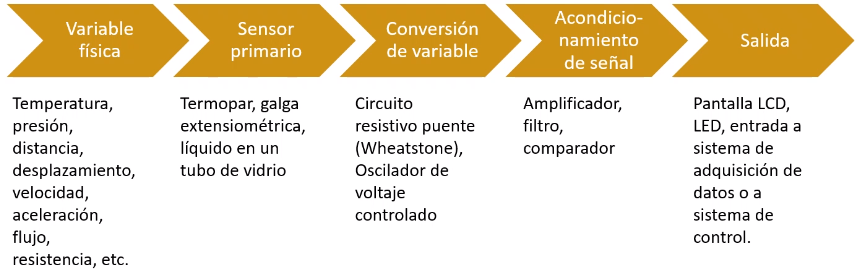
\includegraphics[width=\textwidth]{Media/diagrama_sistemas_de_mediciones.png}
    \caption{Diagrama de sistemas de mediciones.}
    \label{Fig: Diagrama de sistemas de mediciones}
\end{figure}

\newSubSubSection{Instrumentación y clasificación de los instrumentos}

La instrumentación es el arte de medir el valor de algunos parámetros presentes en algún proceso, como presión, flujo, nivel o temperatura, por nombrar algunas, y devolver una señal que es proporcional al parámetro medido. Las señales de salida están estandarizadas y pueden ser procesadas por otro equipos para activar indicadores, alarmas o control automático.

Los instrumentos se pueden dividir en:
\begin{itemize}
    \item Ciegos: cuando no tienen ninguna indicación visible de la lectura tomada.
    \item Indicadores: muestran el valor medido.
    \item Registradores: cuando son capaces de almacenar la información medida, generando un historial de datos.
\end{itemize}

ó
\begin{itemize}
    \item Activos: la cantidad medida (mesurando) modula la magnitud de alguna fuente de poder externa.
    \item Pasivos: la potencia necesaria para generar la señal de salida del instrumento es producida por completo por acción del mesurando.
\end{itemize}

\begin{figure}[h]
    \centering
    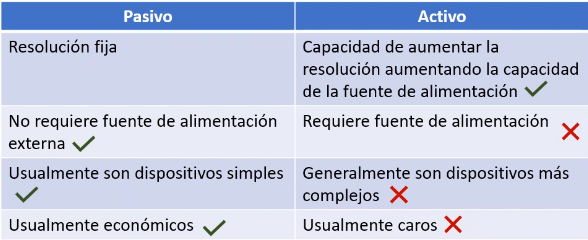
\includegraphics[width=0.5\textwidth]{Media/comparacion_pasivo_activo.png}
    \caption{Comparación de los instrumentos pasivos y activos.}
    \label{Fig: Comparacion de los instrumentos pasivos y activos}
\end{figure}

igual se pueden encontrar:
\begin{itemize}
    \item Instrumentos de deflexión: La variable medida produce en el instrumento un efecto (desplazamiento) y la magnitud del valor medido es desplegado en términos del movimientos producido en el puntero.
    \item Instrumentos nulos: El efecto del mesurando es equilibrado por un efecto opuesto, regresando el sistema a un punto nulo (balanceado). La medición se obtiene de la magnitud opuesta requerida para alcanzar el balance.
\end{itemize}

De igual manera, se pueden dividir en instrumentos análogos y digitales:

Un instrumento análogo entrega una salida que varía (continuamente) de acuerdo a los cambios del mesurando, por ejemplo, el indicador de presión de Bourdon. En principio, la salida puede tener cualquier valor dentro del rango de medición. Un instrumento digital tiene una salida que varía en pasos discretos, por lo que tiene un número fijo de salidas.

\newSubSubSection{Estándares de medición}

\begin{itemize}
    \item Masa: kilogramo (kg).Se define tomando el valor numérico fijo de la constante de Plank.
    \item Longitud: metro (m). Se define tomando el valor numérico fijo de la velocidad de la luz en el vacío.
    \item Tiempo: segundo (s). Se define tomando el valor numérico fijo de la frecuencia del Cesio.
    \item Corriente eléctrica: ampere (A). Se define tomando el valor numérico fijo de la carga elemental.
    \item Temperatura: kelvin (k). Se define tomando el valor numérico fijo de la constante de Boltzmann.
    \item Cantidad de substancia: mole (mol). Se define tomando el valor numérico fijo de la constante de Avogadro.
    \item Intensidad luminosa: candela (cd). Se define con la percepción humana.
\end{itemize}

\newSubSubSection{Conceptos básicos de los instrumentos}

\begin{itemize}
    \item Rango (span): conjunto de valores en la escala de medición dentro de los límites superior e inferior.
    \item Exactitud (accuracy): capacidad del instrumento para acercarse y poder medir el valor real.
    \item Precisión (precision): capacidad del instrumento para obtener el mismo resultado en mediciones diferentes realizadas en las mismas condiciones.
    \item Bias (desplazamiento\footnote{No tiene una traducción literal, se usa desplazamiento como un aproximado.}): es un desplazamiento constante (offset) que se presenta a lo largo de toda la escala de medición del instrumento.
    \item Sensibilidad (sensitivity): razón entra el incremento de la lectura y el incremento de la variable que la ocasiona, después de alcanzar el reposo.
    \item Histéresis (hysteresis): diferencia máxima que se observa en los valores indicados por el instrumento para un mismo valor del campo de medida, cuando la variable recorre toda la escala en for ascendente y luego en forma descendente.
    \item Zona muerta (deadzone): es el intervalo de valores de la variable que no hace variar la indicación o la señal del instrumento, es decir, que no se produce respuesta alguna.
    \item Umbral: nivel mínimo necesario para que el instrumento empiece a indicar una medida, o para que empiece a ser registrado como un cambio.
    \item Resolución: es la mínima subdivisión de la escala.
    \item Incertidumbre: denota la inexactitud del instrumento o la tendencia al error que pueda tener.
\end{itemize}

\newSubSection{Simbología y normatividad}



\newSubSection{Principales criterios para la selección de instrumentos}

Algunos factores para la selección de sensores son:
\begin{itemize}
    \item Características estáticas.
    \item Características dinámicas.
    \item Costo.
    \item Durabilidad.
    \item Mantenimiento.
    \item Compatibilidad.
\end{itemize}

\newSubSubSection{Respuestas de orden cero, primero y segundo}

En los instrumentos con respuesta de \textbf{orden cero}, la salida cambia instantáneamente ante algún cambio en el mesurando como, por ejemplo, el cambio de resistencia en un potenciómetro utilizado para medir desplazamiento.

Los instrumentos con respuesta de \textbf{primer orden} se caracterizan por una constante de tiempo $\tau$. Si el mesurando sufre un cambio abrupto en $\Delta$, $\tau$ es el tiempo que toma a $\Delta$ en cambiar $\approx$ 63\% entre estados inicial y final. La respuesta tiene forma exponencial negativa.

La respuesta de un instrumento de \textbf{segundo orden} es idéntica al comportamiento de un sistema harmónico amortiguado simple. La mayoría de los instrumentos son críticamente amortiguados.

\newSubSubSection{Calibración y trazabilidad}

Los instrumentos solo pueden ajustarse a las características estáticas y dinámicas si están debidamente \textbf{calibrados}. Esto se realiza normalmente de modo jerárquico, calibrando cada instrumento contra otro instrumento similar aún más exacto, cuyo único propósito es calibrar otros instrumentos.

Para la calibración, debe ser posible comprobar una cadena ininterrumpida de comparaciones que termina (o comienza) en algún organismo de estandarización nacional, típicamente algún instituto nacional de metrología como el CENAM. Esta cadena comprobable hacia los estándares internacionales con exactitud conocida se llama \textbf{trazabilidad}.

\newSubSubSection{Procesamiento de señal}

El procesamiento de las señales proveniente de instrumentos de medición se utiliza para mejorar la calidad de la lectura de la señal a la salida del sistema de mediciones o para extraer información útil.

\newSubSection{Error asociado a los intrumentos de medición}

\newSubSubSection{Incertidumbre en las mediciones y otras fuentes de error}

Normalmente se definen do tipos de incertidumbre:
\begin{itemize}
    \item Incertidumbre aleatoria.
    \item Incertidumbre sistemática.
\end{itemize}

La \textbf{incertidumbre aleatoria} se debe a las fluctuaciones (aleatorias) o ruido inherente a la señal. Se presenta muy seguido cuando un humano observa las lecturas de un medidor analógico. Usualmente, la incertidumbre aleatoria se minimiza realizando promedios de las lecturas de alguna manera.

La \textbf{incertidumbre sistemática} es aquella que no se puede corregir mediante el promedio de mediciones repetidas. Generalmente, el error humano está involucrado en los errores sistemáticos. Algunos de los factores que ocasionan errores sistemáticos son: instrumentos mal calibrados, aguja del medidor doblada, lectura humana de un medidor de aguja desde un ángulo (parallax error).

Otras fuentes de error pueden ser:
\begin{itemize}
    \item \textbf{Conexión de puntas de prueba}: es muy común que la resistencia de las puntas de prueba no se tome en cuenta, así como tampoco la dependencia de esta resistencia con respecto a la temperatura. Debe hacerse todo lo posible para minimizar la longitud de las puntas, ya que pueden funcionar como antenas, enviando o (pero aún) captando señales ``perdidas'' como la de la red eléctricas de 60Hz.
    \item \textbf{EMFs térmicas (EMF $\rightarrow$ Fuerza electromotriz)}: siempre que dos metales diferentes se unen, se genera una fuerza.
\end{itemize}

\newSubSubSection{Perturbación de un sisitema debido a las mediciones y características de las señales}

Es imposible realizar mediciones en un sistema sin perturbarlo de alguna manera.

\begin{itemize}
    \item DC (corriente directa), son señales con valores constantes que no cambian con respecto al tiempo.
    \item AC (corriente alterna), son señales senoidales o superposición de las mismas.
\end{itemize}

\newpage
\newSection{Unidad 2: Métodos instrumentales de análisis}

\newSubSection{Adquisición de datos}
\newSubSection{Calibración de los instrumentos de medición}
\newSubSection{Instrumentación virtual}
\newSubSection{Análisis estadístico de los datos}

\newpage
\newSection{Unidad 3: Aplicaciones de los microcontroladores en sistemas de instrumentación}

\newSubSection{Adquisición de datos a través de microcontroladores}
\newSubSection{Procesamiento y análisis de variables físicas para sistemas de adquisición de datos autónomos basados en microcontroladores}
\newSubSection{Control digital aplicado a la instrumentación}
\newSubSection{Protocolos de transmisión de datos utilizando microcontroladores}
\newSubSection{Interfaces para instrumentación virtual basada en microcontroladores}

\newpage
\newSection{Unidad 4: Técnicas modernas para automatización de procesos}

\newSubSection{Dispositivos reconfigurables}
\newSubSection{Niveles de integración de los componentes electrónicos}
\newSubSection{Acondicionadores de señal monolíticos}
\newSubSection{Controladores analógicos integrados}

\end{document}